%% LyX 2.4.2.1 created this file.  For more info, see https://www.lyx.org/.
%% Do not edit unless you really know what you are doing.
\documentclass[12pt,english]{beamer}
\usepackage{mathpazo}
\renewcommand{\familydefault}{\rmdefault}
\usepackage[T1]{fontenc}
% \usepackage[latin9]{inputenc}
\setcounter{secnumdepth}{3}
\setcounter{tocdepth}{3}
\usepackage[active]{srcltx}
\usepackage{amsthm}
\usepackage{amssymb}
\usepackage[authoryear]{natbib}
\usepackage{graphicx}

\makeatletter
%%%%%%%%%%%%%%%%%%%%%%%%%%%%%% Textclass specific LaTeX commands.
% this default might be overridden by plain title style
\newcommand\makebeamertitle{\frame{\maketitle}}%
% (ERT) argument for the TOC
\AtBeginDocument{%
  \let\origtableofcontents=\tableofcontents
  \def\tableofcontents{\@ifnextchar[{\origtableofcontents}{\gobbletableofcontents}}
  \def\gobbletableofcontents#1{\origtableofcontents}
}
\theoremstyle{definition}
\newtheorem*{example*}{\protect\examplename}
\theoremstyle{definition}
\newtheorem*{defn*}{\protect\definitionname}
\theoremstyle{plain}
\newtheorem*{thm*}{\protect\theoremname}

%%%%%%%%%%%%%%%%%%%%%%%%%%%%%% User specified LaTeX commands.
\AtBeginDocument{%
   \let\origtableofcontents=\tableofcontents
   \def\tableofcontents{\@ifnextchar[{\origtableofcontents}{\gobbletableofcontents}}
   \def\gobbletableofcontents#1{\origtableofcontents}
 }\usepackage[english]{babel}
\usepackage{babel}

%\usetheme{Boadilla}
\usetheme{Madrid}
\setbeamertemplate{navigation symbols}{}
% \usecolortheme{orchid}
\usecolortheme{spruce}
% \usecolortheme{beaver}

\setbeamercovered{transparent}

\usepackage{colortbl}

\usefonttheme[onlymath]{serif}
%%%%%%%%%%%%%%%%%%%%%%%%

% For tables
\usepackage{multirow}
\usepackage{array}
\usepackage{rotating}
\usepackage{longtable}
\usepackage{float}
\usepackage{booktabs}


% For figures
\usepackage{caption}
\usepackage{subcaption}

\makeatother

\usepackage{babel}
\providecommand{\definitionname}{Definition}
\providecommand{\examplename}{Example}
\providecommand{\theoremname}{Theorem}

\begin{document}


\title[MLE]{Maximum Likelihood}

\makebeamertitle






\begin{frame}[plain]{Scientific Reasoning}
\begin{center}
    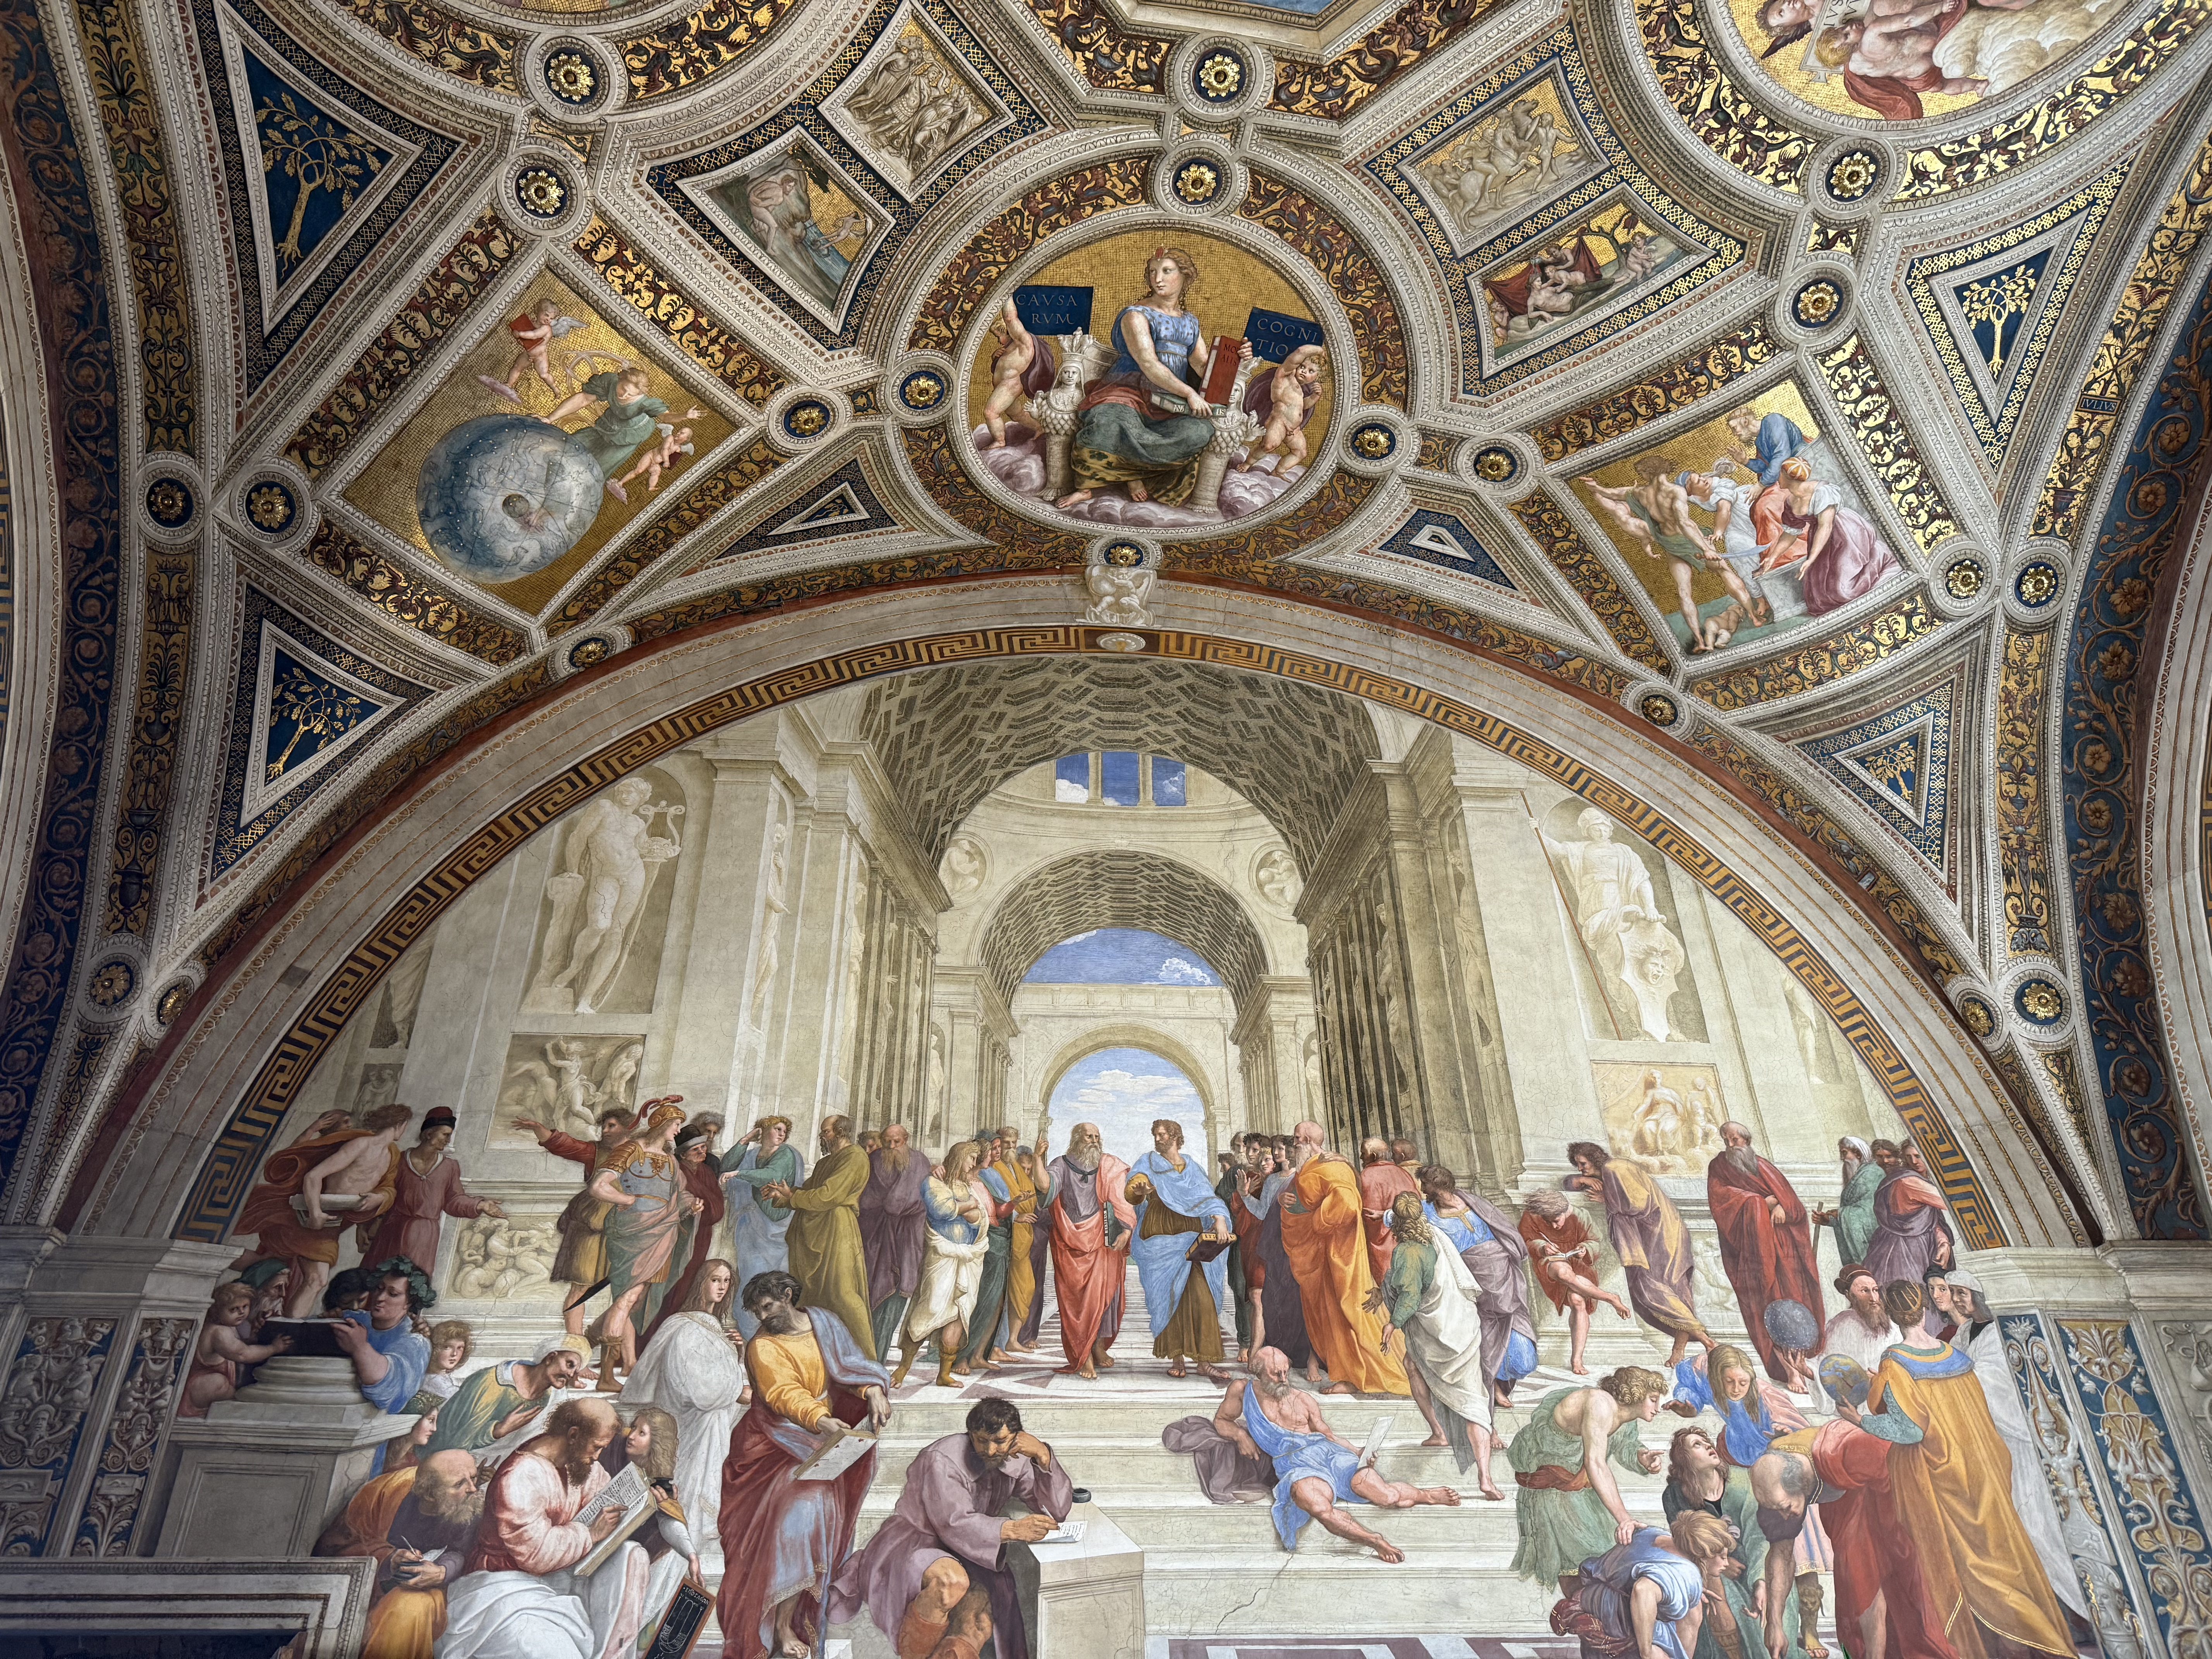
\includegraphics[width=\textwidth]{fig/The_School_of_Athens.jpg}
\end{center}
\end{frame}



\begin{frame}[plain]{Deductive Reasoning}
    \begin{center}
    \includegraphics[width=\textwidth]{fig/black-hole.jpg}
\end{center}
\end{frame}


\begin{frame}[plain]{Inductive Reasoning}
    \begin{center}
    \includegraphics[width=\textwidth]{fig/AI.jpg}
\end{center}
\end{frame}


\begin{frame}{Where is Econometrics Going?}
    \begin{minipage}{0.4\textwidth} % Left side for text
        Covered topics
        \begin{itemize}
            \item Linear models
            \item OLS
            \item Endogeneity
            \item 2SLS, GMM
        \end{itemize}
        \bigskip

        We will continue...
    \end{minipage}%
    \hfill
    \begin{minipage}{0.5\textwidth} % Right side for image
        \centering
        \includegraphics[width=\textwidth]{fig/30hill.jpg}
    \end{minipage}
\end{frame}




\begin{frame}{In the Era of AI}
    \begin{itemize}

        \item Is econometrics a hard subject?
        \pause \bigskip

        \item Many steps of data analysis
        \item Automating routine tasks
        \begin{itemize}
            \item Coding and data cleaning  
            \item Factual math derivation
        \end{itemize}
        \pause
        \bigskip
        \item Domain knowledge: Interpretation
        \item Understanding the big picture
        \item What if AI suggests something completely new to you?
        \pause \bigskip
        \item Welcome to the beautiful new world of AI.
    \end{itemize}
\end{frame}



\end{document}
